%

\documentclass[aps,longbibliography,final,prl,onecolumn,superscriptaddress,nofootinbib,floatfix,11pt]{revtex4-1}
\usepackage{amsfonts,amssymb,stmaryrd,latexsym,amsmath,braket}
\usepackage{subfigure,graphicx}
\renewcommand{\baselinestretch}{1.0}

\DeclareMathOperator{\sgn}{sgn}

\begin{document}

\noindent

\subsection{Lee research group}
The Lee research group is interested in developing new algorithms for quantum state preparation and time evolution that are sufficiently robust to operate on noisy near-term devices.  These include both digital quantum computers and analog quantum simulators.  The problems we address are designed to probe correlations in nuclear structure, the spectrum of nuclear energy levels, transition matrix elements, and the dynamics of nuclear scattering and reactions.  Ph.D. student Jacob Watkins has worked on the topics presented in this proposal and funds would be used to support his continuing research in quantum computing applied to nuclear physics.  

 
\subsubsection{Variational adiabatic evolution}



In order to perform calculations of the properties of nuclear systems via quantum computing, we need to be able to prepare quantum states in an eigenstate of the nuclear Hamiltonian. The method of adiabatic evolution is one approach to quantum 
 state preparation \cite{Farhi:2000a}.  The adiabatic theorem tells us that if we start in an eigenstate of some time-dependent Hamiltonian $H(t)$, then we remain in an eigenstate of $H(t)$ so long as the time dependence is sufficiently slow and we do not pass through level crossings.  Let us start with some simple Hamiltonian $H_z$ whose ground state $\ket{\phi^0_z}$  can be prepared simply using single qubit gate operations. Suppose we want to produce the
ground state $\ket{\phi^{0}_\odot}$ for some nontrivial Hamiltonian $H_\odot$.  We can define a time-dependent Hamiltonian $H(t)$ so that $H(0)=H_z$ and $H(\tau)=H_\odot$.  If the time dependence is sufficiently slow
and we do not pass through any level crossings, then we obtain an accurate representation of $\ket{\phi_\odot}$ after reaching time $t = \tau$,
\begin{equation}
\ket{\phi_\odot^0} = T \exp\left[-i\int_0^\tau H(t) dt \right]\ket{\phi_z^{0}}.
\end{equation}  In practice, however, decoherence on near-term devices means that the amount of time evolution is severely limited.  This problem is substantially ameliorated for an analog quantum simulator.  However, there remains a general problem of dealing with the errors generated by imperfect adiabatic evolution.    

The strategy of variational adiabatic evolution is to produce a subspace of states corresponding to different time-dependent Hamiltonians $H_{n}(t)$.  We construct the time-evolved state $\ket{\psi_n} = U_n\ket{\phi_z^0}$, where $U_n$ is 
\begin{equation}
U_n = T \exp\left[-i\int_0^\tau H_n(t) dt \right] \label{adiabatic}.
\end{equation}
 This unitary operation can be implemented in small time steps using the Trotter approximation. In order to compute the inner product $\braket{\psi_n|\psi_m}$ and amplitude $\braket{\psi_n|H_\odot|\psi_m}$ we use one auxiliary qubit.  We initialize the auxiliary qubit as $\ket{0}$ while the main system is prepared in the state $\ket{\phi_z^0}$.  We perform a Hadamard transform on the auxiliary qubit and implement controlled unitary gate operations to obtain     
\begin{equation}
\ket{0}\ket{\phi_z^0} \rightarrow (1/\sqrt{2}\ket{0} +1/\sqrt{2}\ket{1})\ket{\phi_z^0}
\rightarrow 1/\sqrt{2}\ket{0}U_n\ket{\phi_z^0} +1/\sqrt{2}\ket{1}U_m\ket{\phi_z^0}.
\end{equation}In order to compute the inner  product $\braket{\psi_n|\psi_m},$ we measure the expectation value of $\sigma_x$ plus $i$ times $\sigma_y$ upon the auxiliary qubit.
In order to compute the amplitude $\braket{\psi_n|H_\odot|\psi_m}$, we measure measure the expectation value of $\sigma_x \otimes H_\odot$ plus $i$ times $\sigma_y \otimes H_\odot$.
Equipped with the inner products $\braket{\psi_n|\psi_m}$
and amplitudes $\braket{\psi_n|H_\odot|\psi_m}$, we can now solve for the variational ground state of $H_\odot$ in the subspace spanned by the vectors $\ket{\psi_n}$. 

We propose to test the variational adiabatic evolution method for a particle on a one-dimensional lattice of length $2L+1$ with an attractive short-range potential at the center of the chain.  We can write the pieces of the Hamiltonian as     
\begin{align}
H_z &= \sigma_z^{(L)}, \\
H_{\rm even} &= \frac{1}{2} \sum_{n=0,2,\cdots,2L-2} [\sigma_x^{(n+1)}\sigma_x^{(n)}
+ \sigma_y^{(n+1)}\sigma_y^{(n)}], \\
H_{\rm odd} &= \frac{1}{2} \sum_{n=1,3,\cdots,2L-1} [\sigma_x^{(n+1)}\sigma_x^{(n)}
+ \sigma_y^{(n+1)}\sigma_y^{(n)}], \\
H_\odot &= H_z + H_{\rm even} + H_{\rm odd}.
\end{align}
In order to describe the physics of a single particle, we consider the linear space where exactly one qubit is in the $\ket{1}$ state and the remaining $2L$ qubits are in the  $\ket{0}$ state.  For $L_t$ time steps and total evolution time $\tau$, we define the time interval $dt=\tau/L_t$.  We let the unitary operator at time step $n_t$ be
\begin{equation}
U(n_t,L_{t},dt) = \exp(-iH_{\rm odd}n_tdt/L_t)\exp(-iH_{\rm even}n_tdt/L_t)\exp(-iH_ zdt).   
\end{equation} 
We will work with the evolved state,
\begin{equation}
\ket{\psi,\tau,L_t} = U(n_t,L_{t},dt) \cdots U(2,L_{t},dt)U(1,L_{t},dt)\ket{\phi_z^0}. 
\end{equation}

We have done some preliminary work to show that this method appears viable. The exact ground state energy of $H_\odot$ in the limit $L \rightarrow \infty$ is $-\sqrt{2}$.  For $L = 100$ the energy to four significant digits is $-1.414$. If we use the parameters $\{\tau = 1.0,L_t = 4\},$ we find that the energy expectation value of $\ket{\psi,\tau,L_t}$ is $-0.973$.  This is not an accurate estimate of the ground state energy, but as good as one might achieve with current digital quantum computing technology.  If we now apply variational adiabatic evolution with two different trajectories, $\{\tau = 1.0,L_t = 4\}$ and $\{\tau = 1.5,L_t = 4\},$ we get a variational energy of $-1.364$.  We see that there is significant improvement as the variational approach is able to remove some contamination from other low-lying energy states. If we now apply variational adiabatic evolution with three different trajectories, $\{\tau = 1.0,L_t = 4\}, \{\tau = 1.5,L_t = 4\},$ and $\{\tau = 2.0,L_t = 4\}$, we get a variational energy of $-1.399$.  The method appears to be converging rapidly with the number of variational states.   

We propose to study the convergence rate and error stabilization of variational adiabatic evolution for our quantum particle bound to a potential for various values of $L$.  We first analyze the system using standard classical computing with simulation software such as Qiskit.  We then work with our collaboration partners to implement on digital quantum computing devices  at Google and IBM Q.  We will compare with standard adiabatic evolution as well as the quantum approximate optimization algorithm \cite{Farhi:2014}. We will vary the number of particles, $N$, and vary the width of the trapping potential in $H_z$.  Our many-body system will correspond to $N$ identical spinless fermions in a one-dimensional trap.  For $L = 40$ and $N = 20$ the number of possible quantum states will exceed $10^{11}$.

Perhaps the most important aspect of this project is error stabilization.  The inner products $\braket{\psi_n|\psi_m}$ and amplitudes $\braket{\psi_n|H_\odot|\psi_m}$ will suffer from noise.  The first step is to remove any systematic biases using known extrapolation methods \cite{Kandala:2019}. For the remaining error we apply new tools that we have recently developed for another computational technique called eigenvector continuation \cite{Frame:2017fah}.  The error stabilization algorithm involves Monte Carlo simulations of the data with estimated errors included, while throwing out trials that do not satisfy physically-motivated conditions such as norm positivity and constraints on level ordering. 
    
If we add a complex Gaussian error with width $0.05$ to each of the inner products $\braket{\psi_n|\psi_m}$ and amplitudes $\braket{\psi_n|H_\odot|\psi_m}$ in our previous variational calculation with three trajectories, then our error stabilization algorithm gives an estimate of $-1.51(24)$. If error size is reduced to $0.02$, the estimate is $-1.46(12)$. For an error of size $0.01$ the estimate is $-1.41(7)$.  We propose to make further improvements to the error stabilization algorithm by studying the behavior of eigenvectors and eigenvalues under noise perturbations.  We will investigate both the underlying theory and its practical implementation. 

\subsubsection{Spectral reconstruction and transition matrix elements}
     
Quantum phase estimation is one approach to computing the spectrum of a Hamiltonian through real-time evolution and the inverse quantum Fourier transform \cite{Abrams:1999}.  We propose to investigate a different approach that can compute the low-lying excitation spectrum of a quantum system without the use of auxiliary qubits.  The steps are as follows.  We first prepare the state $\ket{\psi}$ using imperfect adiabatic evolution, as we have discussed in the text surrounding Eq.~(\ref{adiabatic}). We can write $\ket{\psi}$ as a linear combination of eigenstates of 
 $H_\odot$,
\begin{equation}
\ket{\psi} = \sum_n c_n \ket{\phi^n_\odot}.
\end{equation}The strategy is to prepare $\ket{\psi}$ so that the sum is dominated by only a few low-lying eigenvectors. 



Let $O$ be some Hermitian operator that does not commute with the Hamiltonian and thus induces  transitions between energy eigenstates.  For example, $O$ could be an electric multipole operator for a nuclear system. We evolve the state $\ket{\psi}$ for a sequence of equally-spaced times $t$,
\begin{equation}
\ket{\psi(t)} = \exp(-iH_{\odot}t) \ket{\psi}.
\end{equation}
We measure the expectation value of $O$ for each $t$, 
\begin{equation}
\braket{O(t)} = \braket{\psi(t)| O |\psi(t)}. 
\end{equation}
In terms of the energy eigenstates, the expectation value is 
\begin{equation}
\braket{O(t)} =   \sum_{n'}  \sum_n c^*_{n'} c_n \braket{\phi^{n'}_\odot|O|\phi^n_\odot}
e^{-i(E^{n}_\odot-E^{n'}_\odot)t},
\end{equation}
where $E^{n}_\odot$ is the energy corresponding to $\ket{\phi^n_\odot}$.
Using a classical computer, we now calculate the Fourier transform of $\braket{O(t)}$.  From the Fourier transform we can extract the energy differences $E^{n}_\odot-E^{n'}_\odot$.  This gives us the excitation energies
of all low-lying states with non-negligible overlap with $\ket{\psi(t)}$.

We propose to develop the efficiency of this spectral reconstruction technique by exploring various transition operators $O$ and various imperfectly-evolved states  $\ket{\psi(t)}$ that maximize the transition  of each excited state to the ground state.
We have done some preliminary work to show that this method is viable for analog quantum simulators.  As an example we consider the so-called time fractal system of trapped ions as described in Ref.~\cite{Lee:2019gtc}.  Similar to atomic nuclei, this system has a rich spectrum of bound states.  The bound state energies form a geometric sequence as a consequence of discrete scale invariance.   


We consider a one-dimensional chain of ions in
a radio-frequency
trap with qubits represented by two hyperfine ``clock''
states.  Such systems have been pioneered by the Monroe group using   $^{171}$Yb$^{+}$ ions  \cite{Zhang:2017a,Zhang:2017b}.
  Off-resonant laser beams are used
to drive stimulated Raman transitions for all ions in the trap.  This induces
effective interactions between
all qubits with
a power-law dependence on separation distance.
 We define the vacuum state as the state  with $\sigma_z^{(n)}=1$ for all sites $n$.
 We use interactions of the form $\sigma_x^{(n)}\sigma_x^{(n')}+\sigma_y^{(n)}\sigma_y^{(n')}$,
to achieve the hopping of spin excitations.  We then use a
$\sigma_z^{(n)}\sigma_z^{(n')}$ interaction to produce  a two-body potential
felt by pairs of spin excitations, and we also consider an external one-body
potential coupled to $\sigma_z^{(n)}$. 

We can view each spin
excitation  with $\sigma_z^{(n)}=-1$ as a bosonic particle
at site $n$ with hardcore interactions preventing multiple occupancy.   In
this language, the Hamiltonian we consider  has the form 
\begin{align}
H =\frac{1}{2} \sum_{n}\sum_{n'\ne n} J_{nn'}[b^{\dagger}_n b_{n'} +b^{\dagger}_{n'}
b_n] & + \frac{1}{2}\sum_{n}\sum_{n' \ne n}V^{}_{nn'}b^{\dagger}_n b_n b^{\dagger}_{n'}
b_{n'} \nonumber\\
& + \sum_{n}U^{}_{n}b^{\dagger}_n b_n+C, \label{time_fractal}
\end{align}
where $b_n$ and $b^{\dagger}_n$ are annihilation and creation operators for
the hardcore bosons on site $n$.  The  hopping coefficients $J_{nn'}$ have
the form
$J_{nn} = J_0/|r_n-r_{n'}|^{\alpha}$, where $r_n$ is the position of qubit $n$.  Similarly, the two-body potential coefficients $V_{nn'}$ have the
form $V_{nn'} = V_0/|r_n-r_{n'}|^{\beta}$.   

We now add to $U_n$ a deep attractive potential at some chosen site $n_0$
that traps and immobilizes one boson at that site.  Without loss of generality,
we take the position of that site to be the origin and add a constant to
the Hamiltonian so that the energy of the trapped boson is zero.  We then consider the dynamics
of a second boson that feels the interactions with this fixed boson at the
origin.  In order to produce a quantum system with a geometric spectrum and discrete scale invariance, we choose $\beta=\alpha-1$. As an example, we consider a system with $\alpha = 2$, $\beta = 1$, $J_0 =
-1$, and $V_0
= -30$.  The wave functions for the first twelve even-parity bound states
are shown in Fig.~\ref{even_wavefunctions}. 
We plot
the normalized wave function for $r>0$, where $r$ is measured in lattice
units.
     

\begin{figure}
\centering
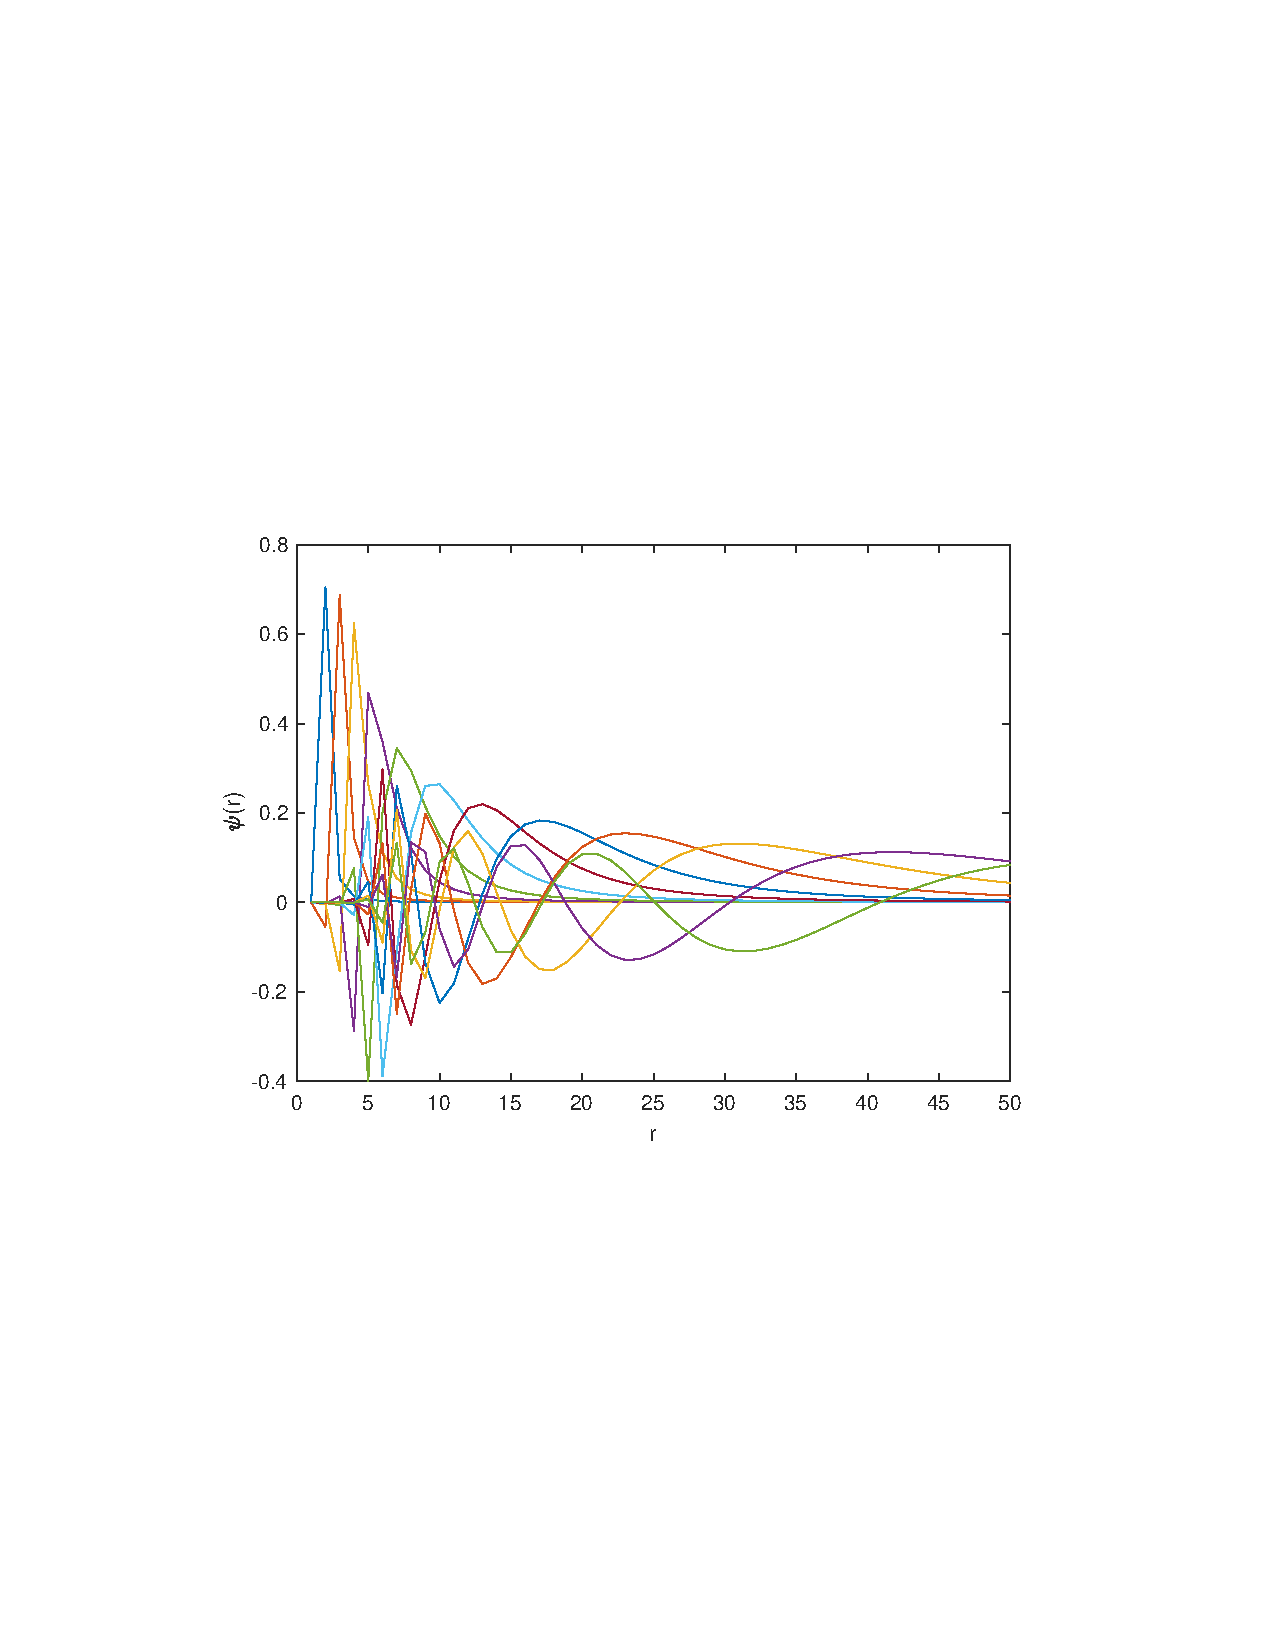
\includegraphics[width=8cm]{v30_even_wavefunctions}
\caption{Plot of the normalized wave functions
for the first twelve even-parity bound states for the case $\alpha = 2$,
$\beta =  1$, $J_0 = -1$,
and $V_0 = -30$.  We plot the region $r>0$, where $r$ is measured
in lattice units.}
\label{even_wavefunctions}
\end{figure}
We propose to reconstruct the excitation spectrum of the time fractal system using 
transition operators of the form $b^{\dagger}_n b_n$ for some particular value of $n$.  This is analogous to the single-nucleon charge density operator.  In addition to the  energy differences $E^{n}_\odot-E^{n'}_\odot$, we can also extract $c^*_{n'} c_n \braket{\phi^{n'}_\odot|O|\phi^n_\odot}$.  Given the fact that $\sum_n |c_n|^2=1,$ this provides a lower bound on the magnitude of the transition matrix element,
$|\braket{\phi^{n'}_\odot|O|\phi^n_\odot}|$. We propose to study different
imperfectly-evolved states $\ket{\psi(t)}$ to generate many different coefficients $c_n$ and thus estimate the magnitude of the transition matrix elements $|\braket{\phi^{n'}_\odot|O|\phi^n_\odot}|$.
  
\subsubsection{Scattering, reactions, and few-body dynamics}
We
propose to study
the real-time dynamics of colliding particles and bound states.  The goal is to provide data from analog quantum simulators that can be used to benchmark state-of-the-art tools used for nuclear scattering and reactions such as the adiabatic projection method \cite{Elhatisari:2015iga}.  For this purpose we use again the time fractal system with Hamiltonian described in Eq.~(\ref{time_fractal}).  In this case, however, we do not include any trapping potential at the center.  Instead we have keep the system uniform except for the open boundary conditions at the ends of the trap.

We have performed preliminary work showing that we can study
the real-time dynamics of colliding particles and bound states
in this manner.  As discussed above, we define the vacuum state as the state  with $\sigma_z^{(n)}=1$ for all
sites $n$.
We can view each spin
excitation  with $\sigma_z^{(n)}=-1$ as a bosonic particle
at site $n$ with hardcore interactions preventing multiple occupancy. If we initialize the system with one particle at the left edge of the ion trap, we can produce a wave packet that moves to the right and bounces elastically off the trap boundaries. In Fig.~\ref{particle} we plot the real-time dynamics of a single particle released from
the left edge of an $L=30$ trap.  We are plotting the particle density for
several time snapshots, with later times linearly displaced in the vertical
direction.

In a similar fashion we can initialize a dimer (two-particle) wave packet by putting two particles on adjacent sites at the edge of the ion trap. In Fig.~\ref{dimer_particle} we plot the real-time dynamics of a dimer and particle released from the left and right edges respectively of an $L=30$ trap.  We are plotting the particle density for
several time snapshots, with later times linearly displaced in the vertical
direction.
 

  The collisions between any $N_1$-body state and $N_2$-body state can be realized in this trapped ion system.  We propose to study how to extract scattering observables from real-time processes on analog quantum simulators.  For elastic scattering we propose to determine reflection and transmission coefficients.  For inelastic scattering we would also like to determine transfer and breakup probabilities for both inclusive and exclusive process. We propose to produce high-quality scattering
and reaction data that can be used to benchmark the adiabatic projection method currently being used for nuclear scattering and reactions in lattice effective field theory.  

\begin{figure}
\centering
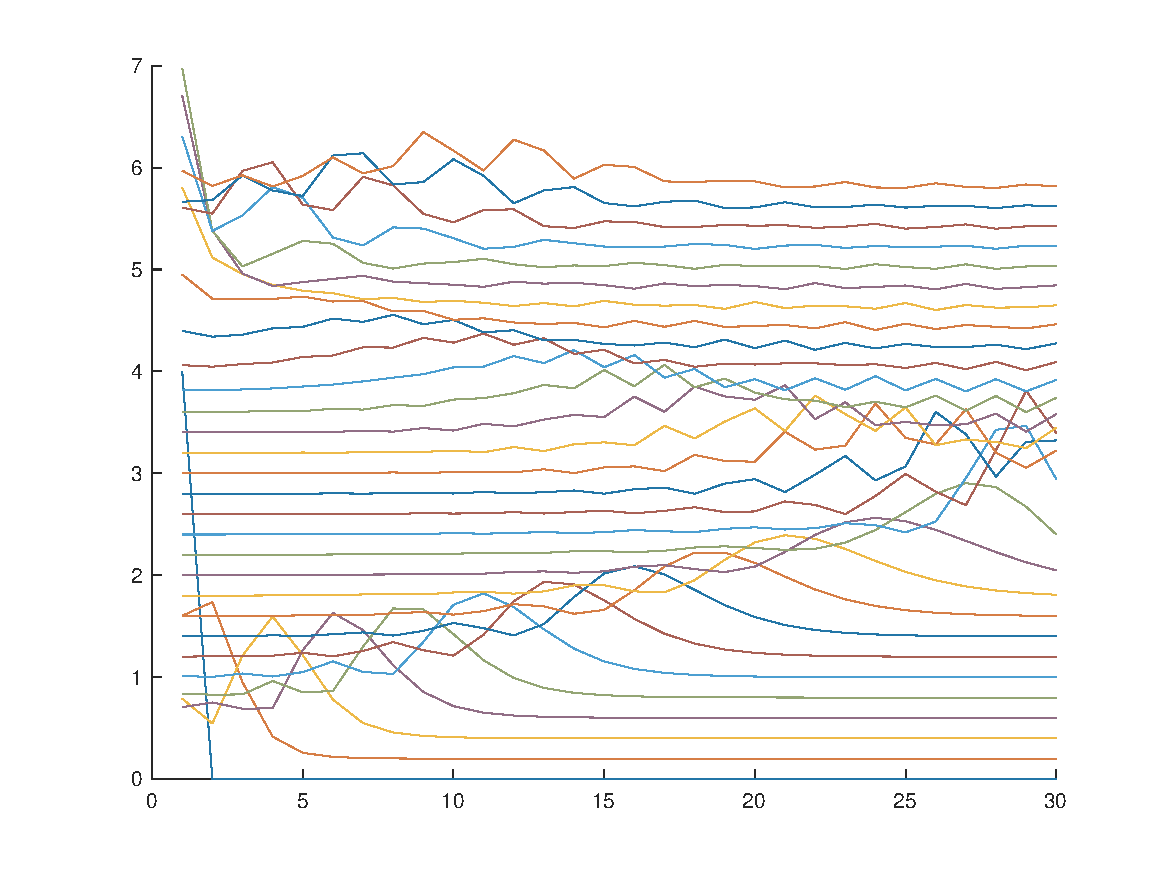
\includegraphics[width=8cm]{particle_1}
\caption{Plot of the real-time dynamics of a single particle released from the left edge of an $L=30$ trap.  We are plotting the particle density for several time snapshots, with later times linearly displaced in the vertical direction.}
\label{particle}
\end{figure}
 
\begin{figure}
\centering
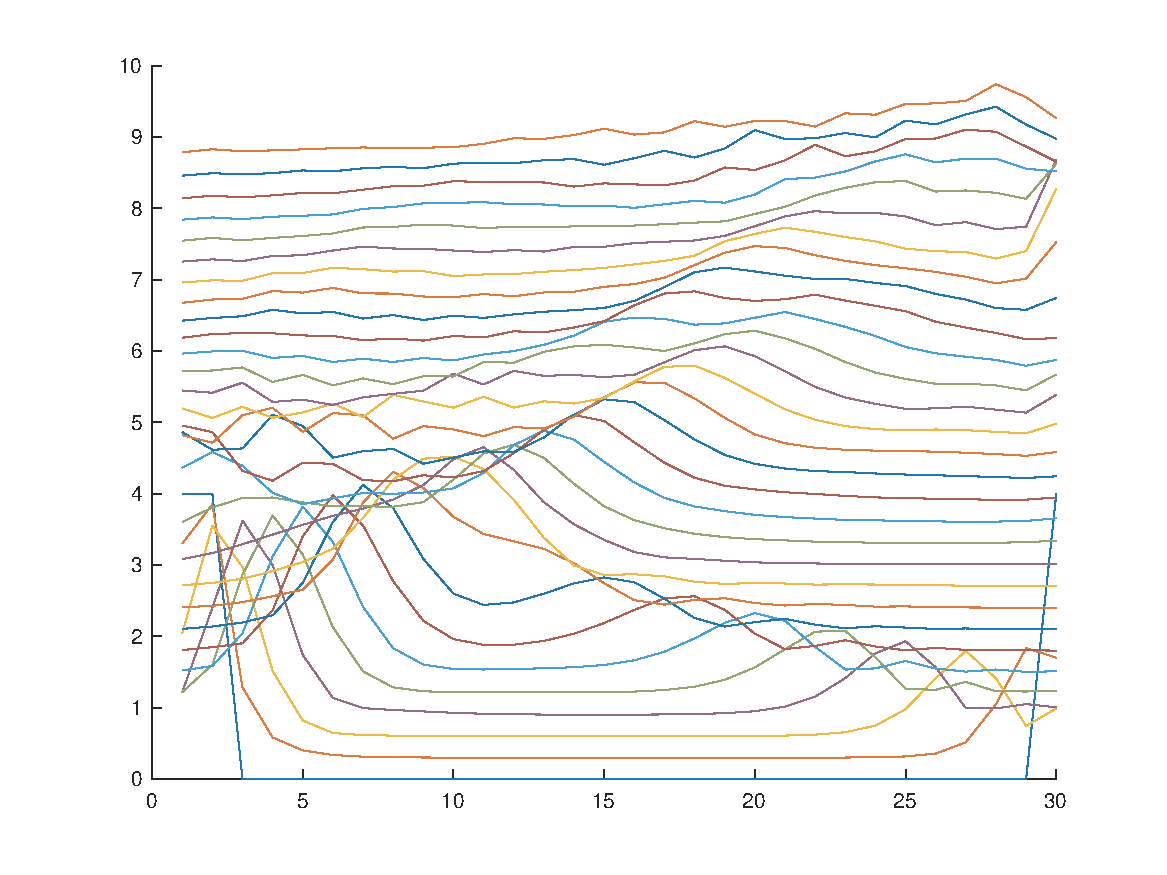
\includegraphics[width=8cm]{dimer_particle_1}
\caption{Plot of the real-time dynamics of a dimer and a single particle released from the left and right edges respectively of an $L=30$ trap.  We are plotting the particle density for
several time snapshots, with later times linearly displaced in the vertical
direction.}
\label{dimer_particle}
\end{figure}
 
\bibliography{References}

\end{document}
 
